%% LaTeX2e class for student theses
%% sections/apendix.tex
%% 
%% Karlsruhe Institute of Technology
%% Institute for Program Structures and Data Organization
%% Chair for Software Design and Quality (SDQ)
%%
%% Dr.-Ing. Erik Burger
%% burger@kit.edu
%%
%% Version 1.1, 2014-11-21



\chapter{Appendix}
\label{chap:appendix}
In this Appendix we present images, complete source code/hybrid program code listings as well as a Glossary at the end.

\section{Images}
\label{app:sec:images}

In the following section different images that have been excluded from the main thesis are presented.

	\begin{figure}[h!]
		\centering
		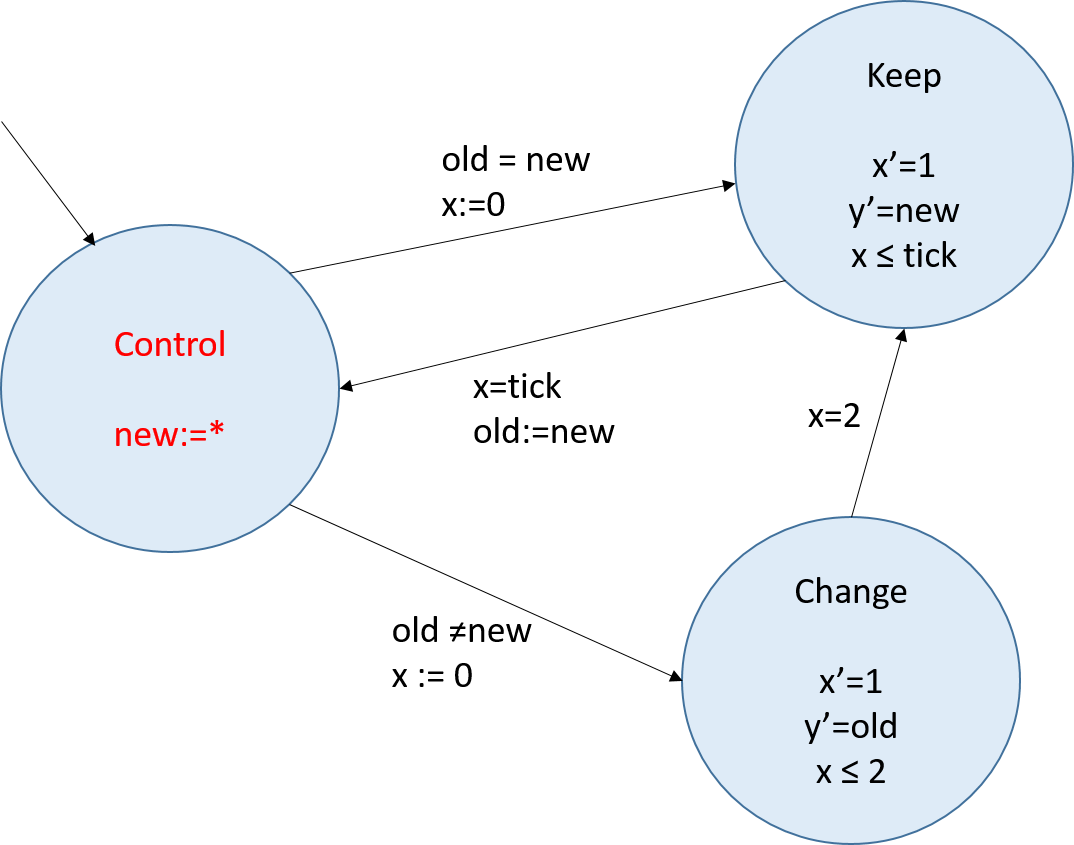
\includegraphics[height=0.5\textheight,width=0.8\textwidth]{Images/ha_control}
		\caption{Watertank Hybrid  Automata with Non-Deterministic Control Program Abstraction marked.}
		\label{fig:ex_control}
	\end{figure}

\section{Negative Acceleration Glue Traffic Control CPS}
\label{app:sec:neg}

As mentioned in Sec.~\ref{subsec:traffic:GlueSpeed} for the fourth component we had to split up the proof into a positive acceleration and negative acceleration part. The glue proof for the negative acceleration can be found below.
\phantomsection
\label{app:eq:traffic1.4.2}
\begin{flalign*}
(x_1 - 1 <  x_j \wedge{}& x_j \leq x_1 \wedge{} \\
v_1 -1 < v_j \wedge{}& v_j \leq v_1 \wedge{} \\
a_1 - 1 < a_j \wedge{}& a_j \leq a_1 \wedge{}\\
v_{sl} - 1 < sl \wedge{}& sl \leq v_{sl} \wedge{} \\
x_{sl} - 1 < slPos \wedge{}& slPos \leq x_{sl} \wedge{} \\
TICK = ep \wedge{}& ep = 2 \wedge{} \\
v_j \geq 0 \wedge{}& v_1 \geq 0 \wedge{} \\
a_j < 0 \wedge{}& a_1 <0 \wedge{} \\
x_j \geq 0 \wedge{}& s_1 \geq 0 \wedge{} \\
sl \geq 0 \wedge{}& v_{sl} \geq 0 \implies{} \\
((x_j < (slPos + 1) \implies{}& (slPos \geq (x_j + 1) + (v_j+1)^2+  \\ 
((((-a_j) + 1) + 1)& * ((-a_j) + 1) * TICK^2 + TICK *(v_j+1)))) \implies{} \\
(x_1 < x_{sl} \implies{}& (x_{sl} \geq x_1 + v_{1}^2+(a_1+1)*(a_1*ep^2+ep*v_1)))))
\end{flalign*}
\section{Listings}
\label{app:sec:listings}

In the following section we present the full java source code for our control program classes, as well as the rule definition we used for \keym. First is the rule definition for \keym, that abstracts the application of the floor function to a inequality of the form \(\textrm{floor}(x) = y \equiv \exists c:x-1 < c \wedge c \leq x \wedge (x \geq 0 \implies c \geq 0) \wedge (x < 0 \implies c < 0)  \longrightarrow\) whereby \(\longrightarrow\) refers to the big implication arrow in the verification of a hybrid program, meaning we get the abstraction of \(f(x)\) on the left side of the implication.

\lstset{language=Java,captionpos=b,tabsize=3,frame=lines,keywordstyle=\color{black},commentstyle=\color{black},stringstyle=\color{black},numbers=left,numberstyle=\tiny,numbersep=5pt,breaklines=true,showstringspaces=false,basicstyle=\footnotesize,emph={label}}
\begin{lstlisting}[label=app:lst:ruleF]
	\rules {
 	 	fdef {
			\schemaVar \term R x;
			\schemaVar \skolemTerm R c;
    			\find(f(x))
			\sameUpdateLevel
			\varcond ( \new(c, \dependingOn(x)) )
			\replacewith(c)
			\add(x-1 < c & c <= x & (x >= 0 -> c >= 0) & (x < 0 -> c < 0) ==> )
			\heuristics(simplify)
		};
	}	
\end{lstlisting}

Next, we provide the full java source code for the Watertank control program class. This means, not only the control method itself is provided, but all the needed class definitions as well.

\lstset{language=Java,captionpos=b,tabsize=3,frame=lines,keywordstyle=\color{blue},commentstyle=\color{darkgreen},stringstyle=\color{red},numbers=left,numberstyle=\tiny,numbersep=5pt,breaklines=true,showstringspaces=false,basicstyle=\footnotesize,emph={label}}
\begin{lstlisting}[label=app:lst:watertankContr]
package watertankSplit;

/**
 * @author Daniel Draper
 * @version 1.0
 * This class is the Watertank's control system.
 */
public class Controller {
	private int tick;
	
	public Controller() {
		tick = 30;
	}
	
	/**
	 * Returns the actual control value for the valve of the watertank.
	 * @param y the current water level
	 * @param old the old valve setting
	 * @return the new valve setting
	 */
	/*@ public normal_behavior
	  @ requires tick == 31 && y >= 10 && y <= 120 && y + 2 * old <= 120 && y + 2 * old >= 10 && (old == 10 || old == -20);
	  @ ensures \result * (tick / 10) + y + 2 * old  >= 12 & \result * (tick / 10) + y + 2 * old <= 116 && (\result == 10 || \result == -20);
	  @*/
	public int getControlValue (int y, int old) {
		//Waterlevel in two time units
		int inTwo = y + 2 * old;
		//If we are raising level, keep raising if possible without hitting max_level before next tick
		if (old == 10) {
			if (inTwo + tick * 1 <= 116) {
				return 10;
			}
			else {
					return -20;
			}
		}
		//ELSE if we are currently lowering level, keep lowering if we can lower further without hitting min_level b4 next tick
		else {
			if (old == -20) {
				if (inTwo - tick * 2 >= 12) {
					return -20;
				}
				else {
						return 10;
				
				}
		
			}
		}
		//Only returned if old != 10 && old != -20, unreachable.
		return 0;
	}
}
\end{lstlisting}

Next, you can find the full source code for the Traffic Control Car Control Program. 

\begin{lstlisting}[label=app:lst:carContr]

package trafficControl;

/**
 * @author Daniel Draper
 * @version 1.0
 * This class models the Car Controller of the Traffic Control CPS.
 */
public class CarController {
	private int TICK;
	private int MAXBREAK;
	private int MAXACCEL;

	public CarController(int TICK, int MAXBREAK, int MAXACCEL) {
		this.TICK = TICK;
		this.MAXBREAK = MAXBREAK;
		this.MAXACCEL = MAXACCEL;
	}
	/**
	 * @param slPos Current Speed Limit Position
	 * @param sl current Speed Limit
	 * @param y current Car Position 
	 * @param v current Car Velocity
	 * @param accel current Car acceleration
	 * @return the new acceleration control Value
	 * The actual control Method.
	 */
	/*@ public normal_behavior
	  @ requires MAXBREAK <= accel - 1 && accel + 1 <= MAXACCEL && v >= 0 && sl >= 0 && TICK == 1 && MAXBREAK == -10 && MAXACCEL == 10 && ((!(y >= slPos - 1)) || ((MAXBREAK+2)*TICK <= ((sl - v) - 2 * TICK))) && ((!(y < slPos + 1)) || (slPos >= (y+1) + (v+1)*(v+1)  + (MAXBREAK + 2 + 1) * ((MAXBREAK + 2) * TICK*TICK + TICK * (v+1))));
	  @ ensures \result - 1 >= MAXBREAK && \result + 1 <= MAXACCEL  && ((!(y >= slPos - 1)) || (\result*TICK <= (sl - v) - 2 * TICK)) && ((!(y < slPos + 1)) || (slPos >= (y+1) + (v+1)*(v+1)  + (\result+ 1 + 1) * ((\result + 1) * TICK*TICK + TICK * (v+1))));
	 @*/
	public int control(int y, int v, int accel, int sl, int slPos) {
		if (y >= slPos - 1 && y < slPos + 1) {
			return MAXBREAK + 1;
		}
		if (y >= slPos - 1) {
			if ((accel+1)*TICK <= (sl-v) - 2 * TICK) {
				if (accel+2 <= MAXACCEL) {
					return accel+1;
				}
				
			}
			else {
				if((accel-1)*TICK <= (sl-v) - 2 * TICK) {
					if (accel-2 >= MAXBREAK) {
						return accel-1;
					}
			}
			}
		}
		if (y < slPos + 1) {
			if (slPos >= (y+1) + (v+1)*(v+1)  + ((accel+1)+1 +1) * ((accel+1 + 1) * TICK*TICK + TICK * (v+1))) {
				if (accel+2 <= MAXACCEL) {
					return accel+1;
				}
			}
			else {
				if (slPos >= (y+1) + (v+1)*(v+1)  + ((accel-1)+1 +1) * ((accel-1 + 1) * TICK*TICK + TICK * (v+1))) {
					if (accel-2 >= MAXBREAK) {
						return accel-1;
					}
				}
			}
		}
			return MAXBREAK + 1;
		
	}
}
\end{lstlisting}

Next, you can find the full source code for the Speed Limit Control Class.
\begin{lstlisting}[label=app:lst:speed]


package trafficControl;


/**
 * @author Daniel Draper
 * @version 1.0
 * This class models the Speed Limit Controller used by the Traffic Control CPS.
 */
public class SpeedLimitController {

	private int TICK;
	private int MAXBREAK;
	private int MAXACCEL;
	/**
	 * @param TICK the Tick duration
	 * @param MAXBREAK the maximum breaking power (<0)
	 * @param MAXACCEL the maximum acceleration (>=0)
	 */
	public SpeedLimitController(int TICK, int MAXBREAK, int MAXACCEL) {
		this.TICK = TICK;
		this.MAXBREAK = MAXBREAK;
		this.MAXACCEL = MAXACCEL;
	}

	/**
	 * @param slPos the current speed limit position
	 * @param sl the current speed limit
	 * @param accel the current car's acceleration value
	 * @param v the current car's velocity
	 * @param y the current car's position
	 * @return both the new speed limit and speed limit position in an array.
	 * The actual control Method.
	 */
	/*@ public normal_behavior
	  @ requires MAXBREAK == -10 && MAXACCEL == 10 && TICK == 1 && v >= 0 && sl >= 0 && ((!(sl < v + 1)) || slPos  >= y+1+ (v+1)*(v+1) + (MAXACCEL + 1 + 1) * ((MAXACCEL+1) * TICK*TICK + TICK * (v+1))) && ((!(sl >= v - 1)) || accel*TICK <= ((sl - v) - 2 * TICK));
	  @ ensures \result[0] >= 0 && ((!(\result[0] < v + 1)) || \result[1]  >= y+1 + ((v+1)*(v+1)) + (MAXACCEL + 1 + 1) * ((MAXACCEL+1) * TICK*TICK + TICK * (v+1))) && ((!(\result[0] >= v - 1)) || accel*TICK <= ((\result[0] - v) - 2 * TICK));
	*/
	public int[] control(int y, int v, int accel, int sl, int slPos) {
		int[] result = new int[2];
		result[0] = sl;
		result[1] = slPos;
		if (sl<25) {
			if (sl+1 < v + 1 && sl+1 >= v - 1) {
				return result;
			}
			if (sl+1 < v + 1) {
				result[0]++;
				result[1] = y+1 + ((v+1)*(v+1)) + (MAXACCEL  + 2) * ((MAXACCEL+1) * TICK*TICK +  TICK * (v+1));
			}
			if (sl+1 >= v -1) {
				if (accel*TICK <= result[0]+1 - v - 2 * TICK) {
					result[0]++;
				}
			}
		}
		else {
			if (sl-1 < v + 1 && sl-1 >= v - 1) {
				return result;
			}
		if (result[0]-1 < v) {
			if (result[0]-1 >= 0) {
			result[0]--;
			
			result[1] = y+1 + (v+1)*(v+1) + (MAXACCEL  + 2) * ((MAXACCEL+1) * TICK*TICK +  TICK * (v+1));
			}
		}
		if (sl-1 >= v - 1) {
			if (accel*TICK <= ((result[0]-1 - v)-2*TICK) && result[0]-1 >= 0) {
				result[0]--;
			}
		}
	}
		return result;

	}
}
\end{lstlisting}
\section{Watertank simulator}
\label{app:sec:simulator}

To be able to execute the watertank control programs and see a result of the computations done on screen (in a form of console output) we had to write a simulator of the differential evolution of the watertank values. The watertank simulator class can be found below:

\begin{lstlisting}[label=app:lst:watertankSim]
package watertankSplit;

/**
 * @author Daniel Draper
 * @version 1.0
 * This class simulates a watertank as modelled in the hybrid model in the KeYmaera Guide.
 */

public class Simulator
{
	private int TICK = 30;
	private Controller contr;
	private int y;
	private int x;
	private int state;
	private int oldDif;
	private int newDif;
	
	/**
	 * Constructs the simulator with correct starting values according to hybrid model.
	 */
	public Simulator() {
		contr = new Controller();
		state = 1;
		y = 10;
		x = TICK;
		oldDif = 10;
		newDif = 10;
	}
	
	/**
	 * One step in the differential evolution of the watertank.
	 */
	private void step() {
		switch (state) {
		case 0:
			if (x == 20) {
				state = 1;
			}
			else {
				y+=oldDif;
				x+=10;
			}
			break;
		case 1:
			if (x == TICK) {
				oldDif = newDif;
				System.out.println("Controlled!");
				newDif = contr.getControlValue(y, oldDif);
				if (newDif == oldDif) {
					state = 1;
					x = 0;
				}
				else {
					state = 0;
					x = 0;
				}
			}
			else {
				y+=newDif;
				x+=10;
			}
			break;
	}
	}
	
	/**
	 * Continuous execution of each timestep and printing the state with an included delay.
	 */
	public void run() {
		do {
			step();
			printState();
				synchronized(this) {		
					try {
						this.wait(500);
					} catch (InterruptedException e) {
						e.printStackTrace();
					}	
					finally {} 
				}
		} while(true);
	}
	/**
	 * Prints the current state of the Watertank.
	 */
	private void printState() {
		System.out.println("Time: " + x/10 + " newDif: " + newDif + " Fillstatus:");
		for (int i = 0; i < y/10; i++) {
		System.out.print("X ");
		}
		for (int i = 0; i < 12 - y/10; i++) {
			System.out.print("_ ");
		}
		System.out.println();
		
	}
	
	/**
	 * Main function creating and executing a new Simulator.
	 * @param args commandline arguments
	 */
	public static void main(String args[]) {
		Simulator s = new Simulator();
		s.run();
	}

}
\end{lstlisting}

\section{Traffic Control Simulator}
\label{app:sec:TrafficSim}

As we did for the Watertank CPS, we also wrote a Simulator for the Traffic Control CPS as to be able to execute the entire program and see the evolution of the car. As the amount of distance between the next speed limit and current car's position can vary greatly, we chose a different way to present the current status of the system than for the watertank, just listing the current status in text form and checking if safety is still guaranteed. It consists of an infinite loop always continuing with one step in the differential evolution of the system, printing the state and an added delay as to make console output readable.

\begin{lstlisting}[label=app:lst:trafficSim]

package trafficControl;

/**
 * @author Daniel Draper
 * @version 1.0
 * This class simulates the environment in the Traffic Control CPS.
 */
public class Simulator {

	private int xDif;
	private int x;
	private int y;
	private int v;
	private int accel;
	private int sl;
	private int slPos;
	private CarController carContr;
	private SpeedLimitController limContr;
	private static int TICK = 1;
	private static int MAXACCEL = 10;
	private static int MAXBREAK = -10;
	
	/**
	 * Creates a new Traffic Control Simulator.
	 */
	public Simulator() {
		xDif = 1;
		v = 10;
		x = 0;
		y = 0;
		slPos = 10;
		sl = 10;
		carContr = new CarController(TICK, MAXBREAK, MAXACCEL);
		limContr = new SpeedLimitController(TICK,MAXBREAK,MAXACCEL);
	}
	
	/**
	 * Starts the entire system, running in an infinite loop.
	 */
	public void run() {
		do {
			printState();
			if (x \% TICK == 0) {
				accel = carContr.control(y,v,accel,sl,slPos);
					int[] res = limContr.control(y,v,accel,sl,slPos);
					sl = res[0];
					slPos = res[1];
			}
			int v0 = v;
			x += xDif;
			v += accel;
			y += (v0 + 0.5 * accel);
				synchronized(this) {		
			try {
				this.wait(500);
			} catch (InterruptedException e) {
				// TODO Auto-generated catch block
				e.printStackTrace();
			}	
			finally {} 
		}
		} while(true);
	}
	/**
	 * Prints the current state of the system.
	 */
	private void printState() {
		System.out.println("We have: Car at Pos. " + y + " with velocity " + v + " and acceleration " + accel);
		System.out.println("Speed limit " + sl + " at Pos. " + slPos);
		System.out.println("If car breaks at max_Break_Speed " + MAXBREAK + " at next tick, car has speed " + (v + accel) + " and afterwards speed " + (v+accel+MAXBREAK));
		if (y >= slPos) {
			if (accel*TICK <= (sl- v)) {
				System.out.println("Safety kept!");
				return;
			}
		}
		else {
			if (2*slPos*MAXBREAK*(-1) >= y*2*(-1)*MAXBREAK + (v*v - sl*sl)  + (accel+(-1)*MAXBREAK) * (accel * TICK*TICK + 2*TICK * v)); {
				System.out.println("Safety kept!");
				return;
			}
		}
		System.err.println("Safety condition not kept!");
	}

	/**
	 * @param args Commandline Arguments.
	 * Main function for execution.
	 */
	public static void main(String[] args) {
		Simulator s = new Simulator();
		s.run();
	}
}
\end{lstlisting}

\section{Complete Hybrid Programs in correct ASCII notation}
\label{app:sec:pdfs}

In this section we present the complete hybrid programs from this thesis. As we mentioned in Ch.~\ref{ch:Preliminary}, hybrid programs have to be typeset in ASCII for \keym~to be able to read it, which is why these hybrid programs look different from the ones we present in the previous chapters. The first two hybrid programs are the original watertank hybrid program and our remodelled version that includes the hook, a suitable postcondition as well as the tick.
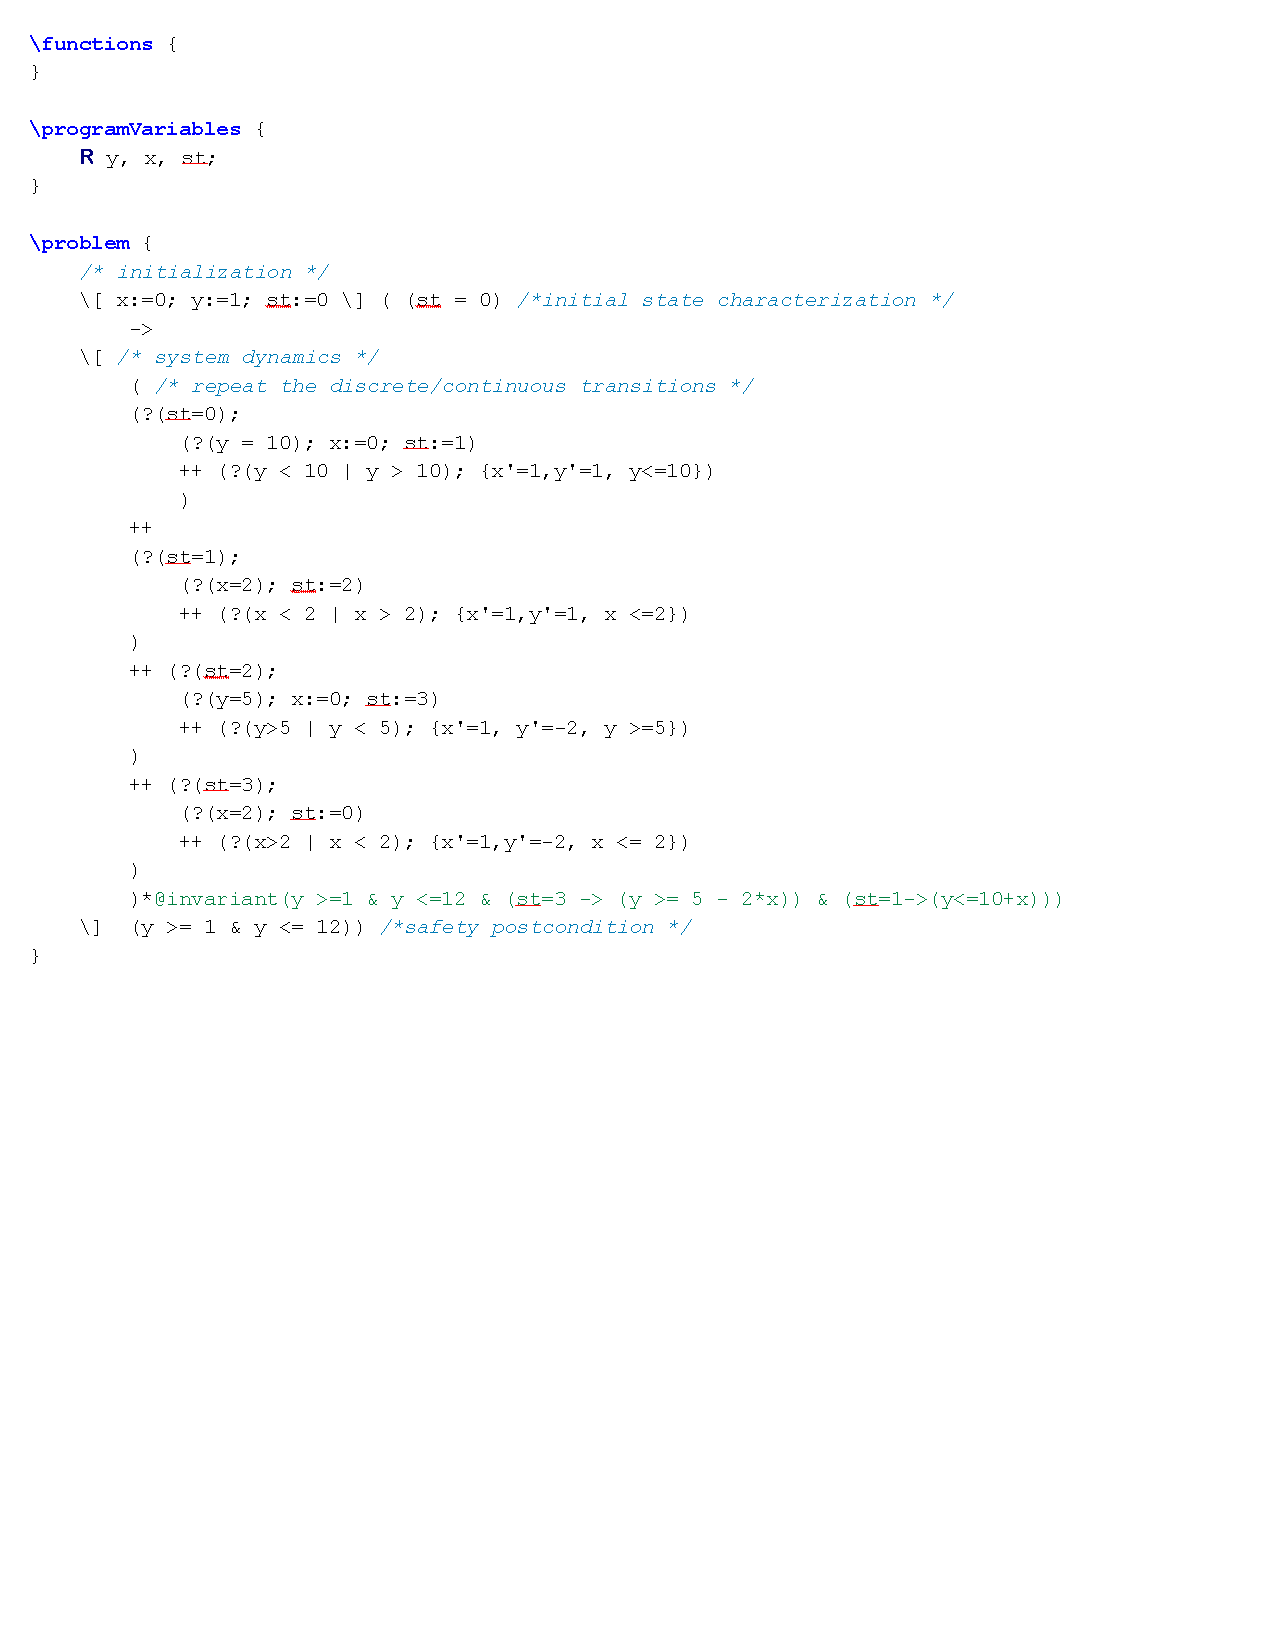
\includepdf[pages=1,scale=1]{images/watertank_hp.pdf}

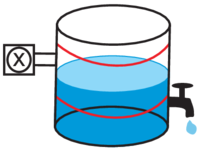
\includepdf[pages=1,scale=1]{images/watertank.pdf}

Next up is the glue proof for the watertank cps typeset in ASCII.

\includepdf[pages=1,scale=1]{images/glue.pdf}

The next two hybrid programs are the original Traffic Control hybrid program, as well as it's remodelled version that includes the hooks (as in this case we have two control programs), the postconditions and a tick.
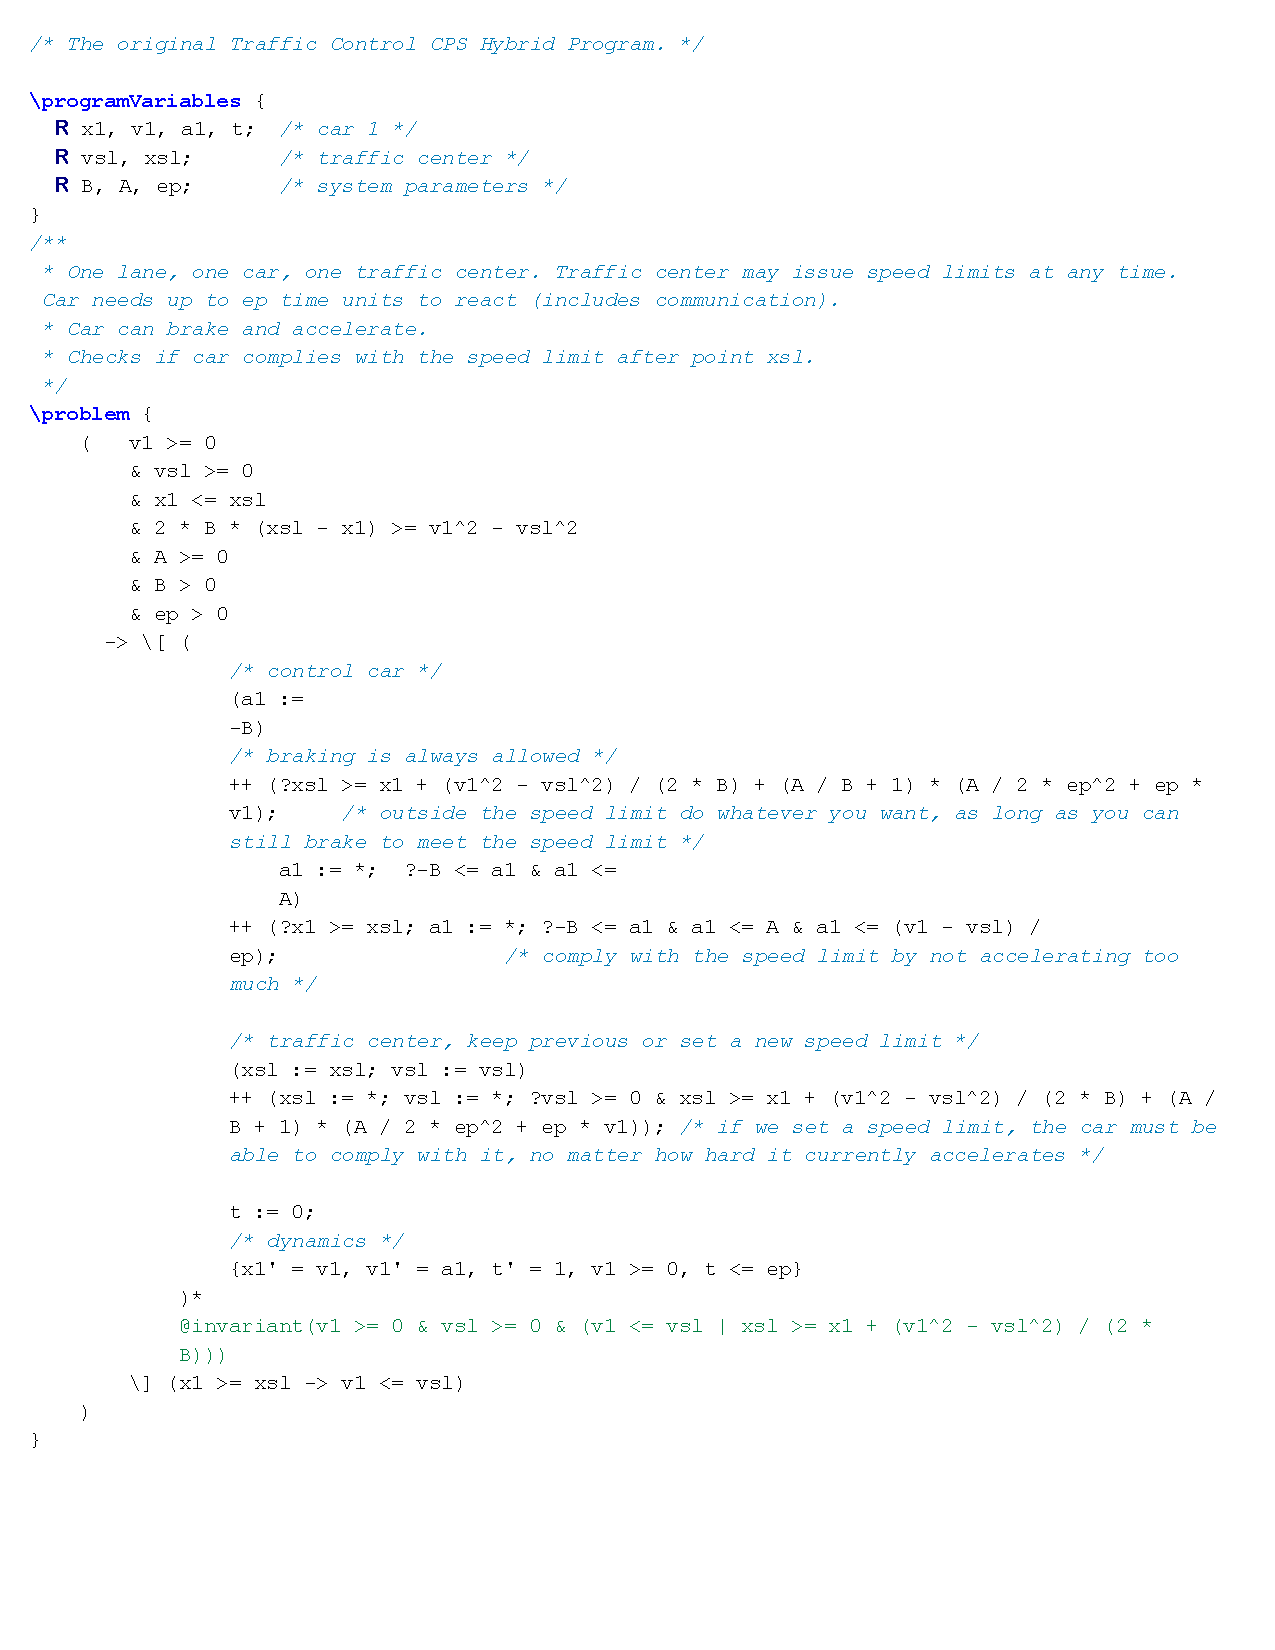
\includepdf[page=1,scale=1]{images/trafficControlOrig.pdf}

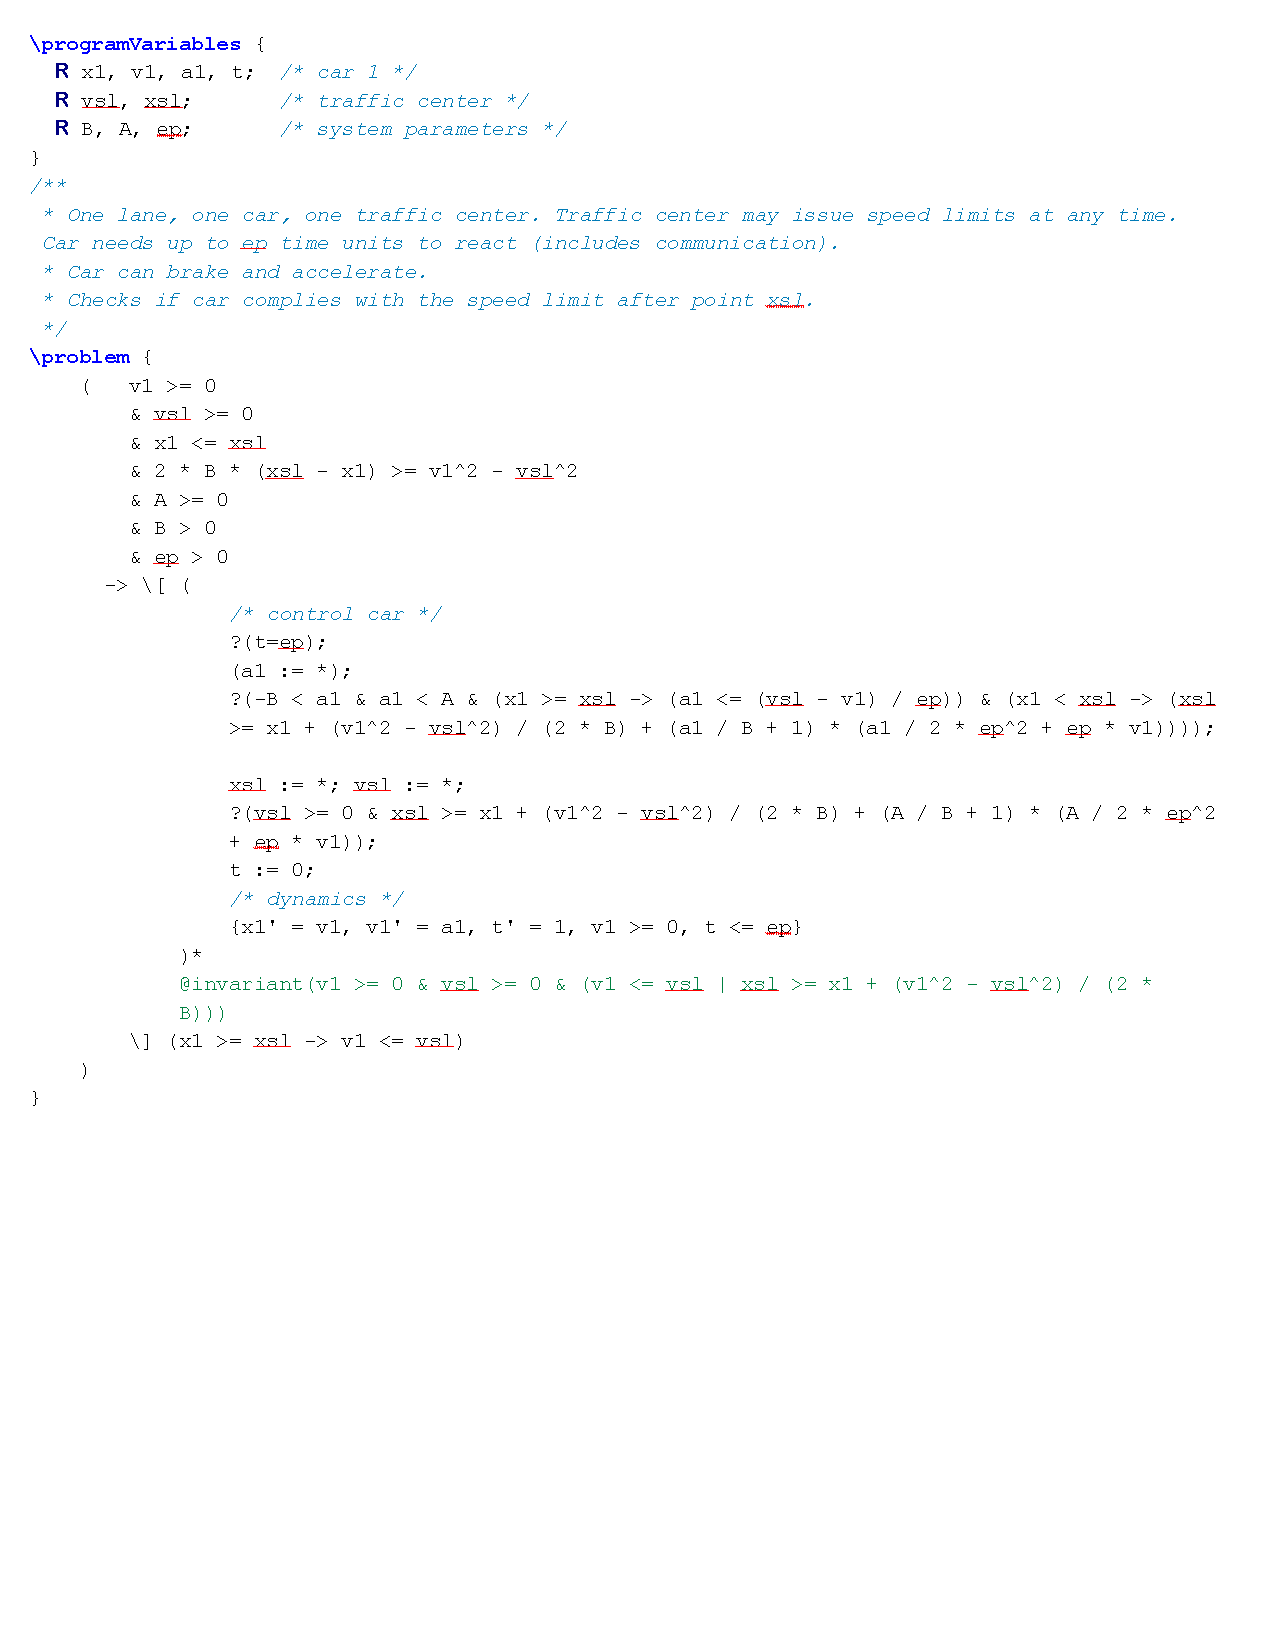
\includepdf[page=1,scale=1]{images/trafficControlRem.pdf}

What now follows is the glue proof for the traffic control cps typeset in ASCII.

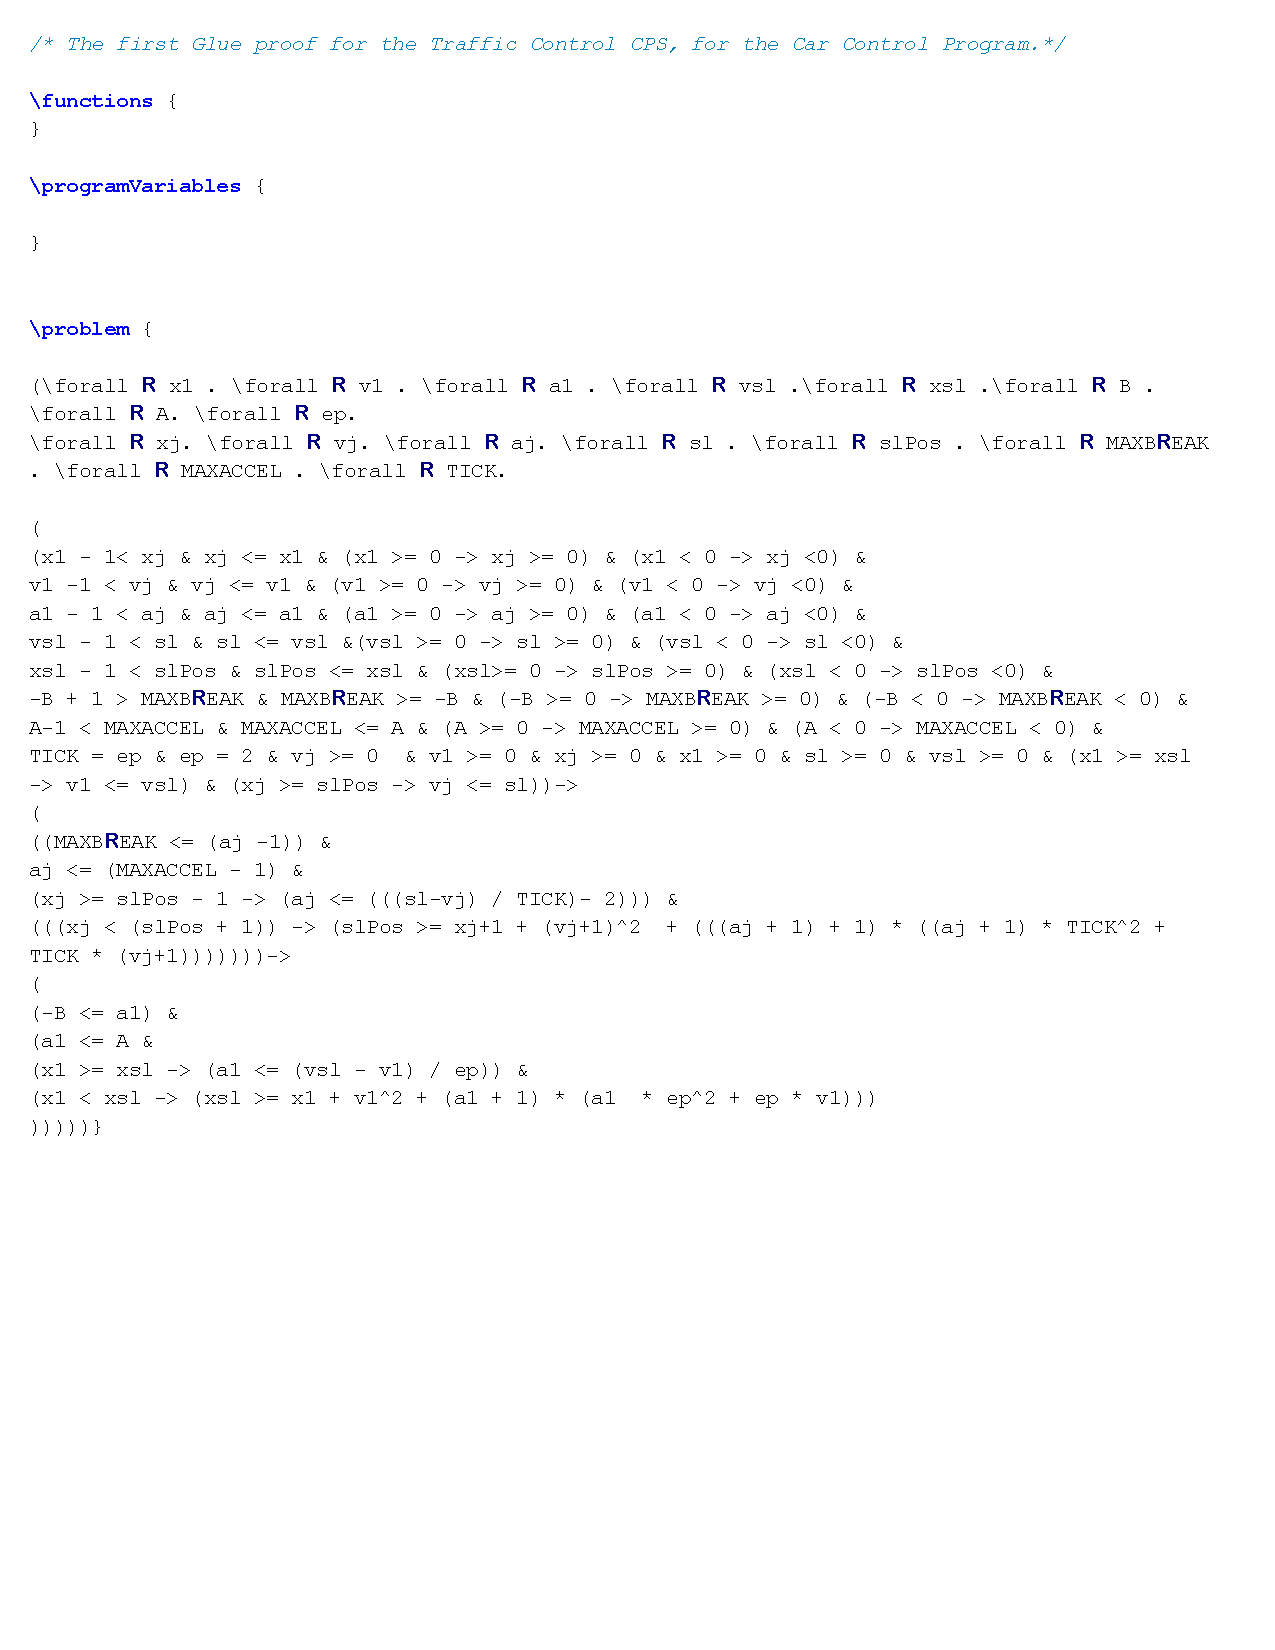
\includepdf[page=1,scale=1]{images/glue_traffic_1.pdf}

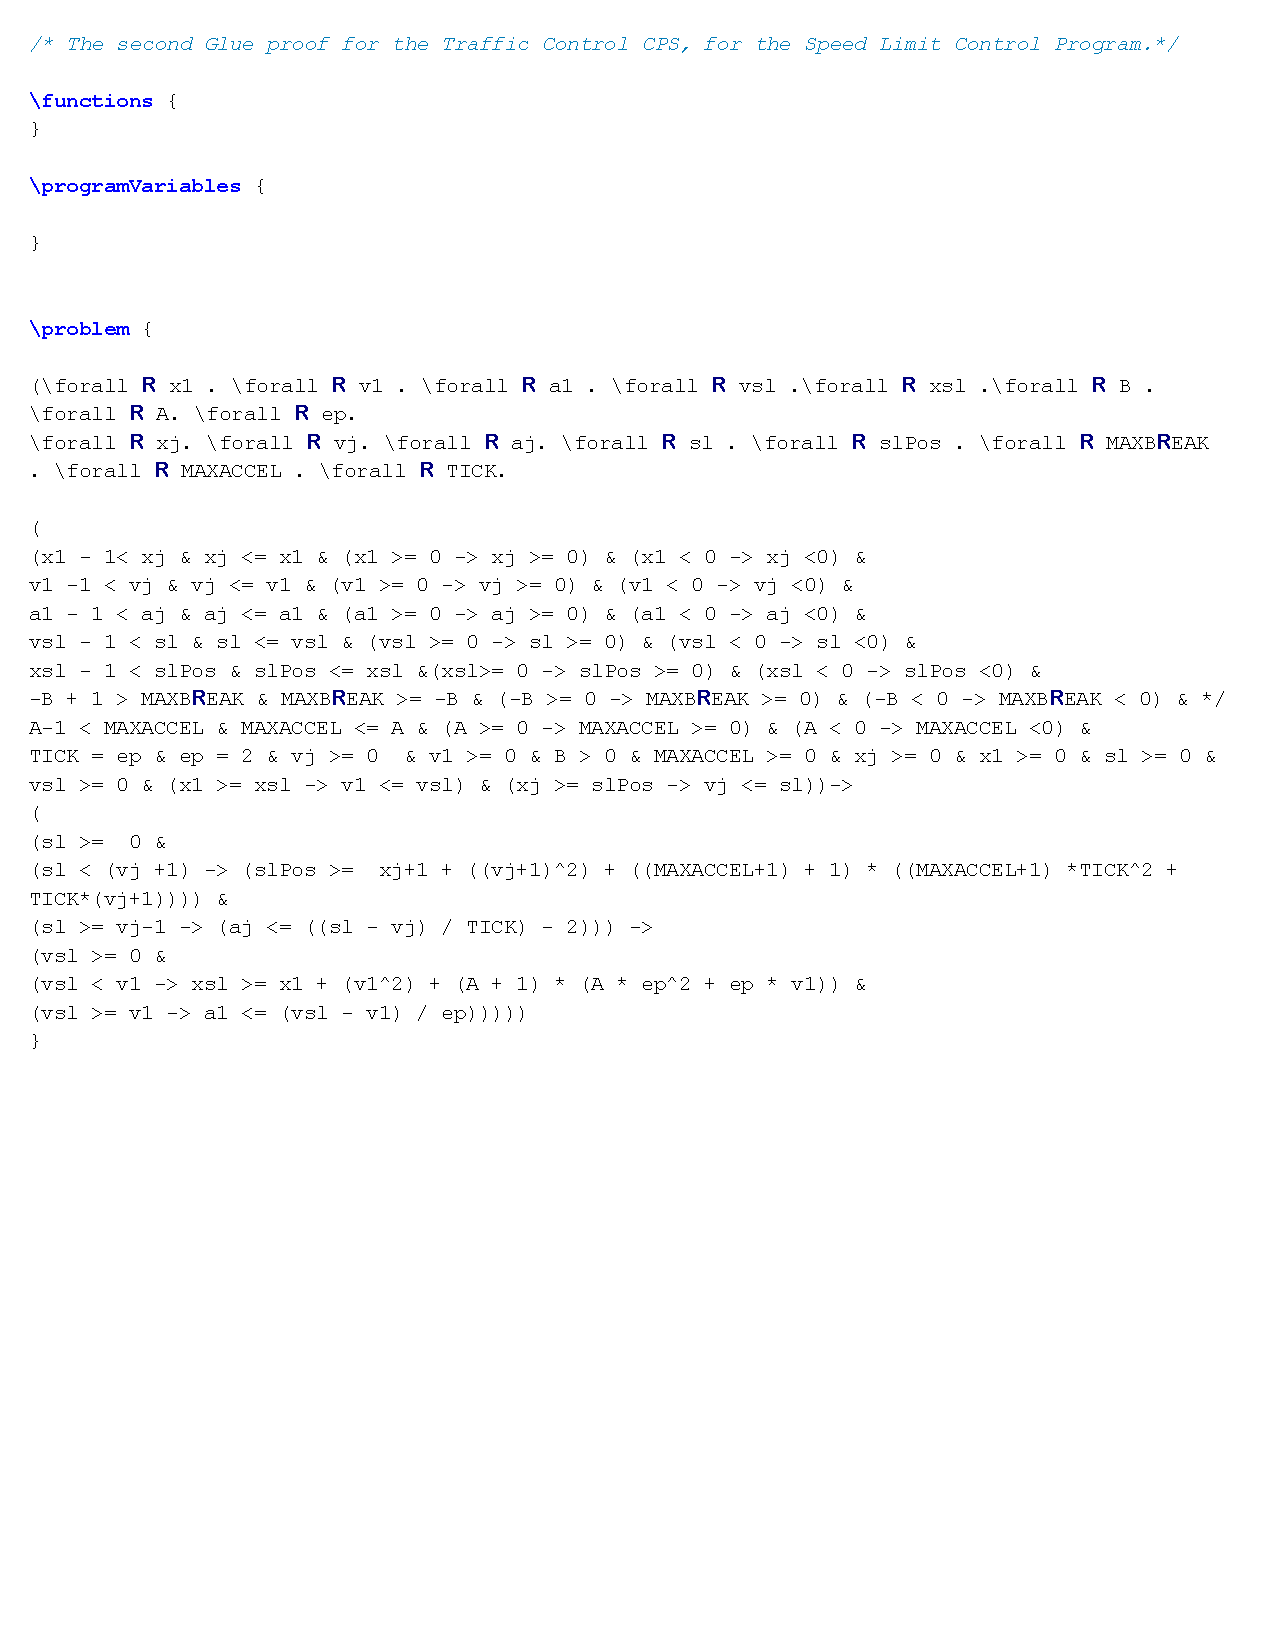
\includepdf[page=1,scale=1]{images/glue_traffic_2.pdf}

\newglossaryentry{cps} {
 name=Cyber-Physical System[CPS],
 description={is a system describing motions or evolutions in which a physical aspect is being controlled by a computer/computer program. In this thesis equivalent to the notion of Hybrid Systems.}
}

\newglossaryentry{hybrid}{
 name=Hybrid System,
 description={is a system in which discrete as well as continuous evolutions are present. E.g, a remote controlled car which can only be accelerated or braked, its movement is continuous and follows continuous differential equations, while the control program is discrete and can only take discrete values (e.g, Acceleration := 1; Acceleration := 2 etc.).}
}

\newglossaryentry{hook}{
name=Hook,
description={refers to a/multiple concrete instruction at which the control program is executed when describing a hybrid system as a hybrid program. This is one or multiple non-deterministic assignments of values, e.g a:=*.}
}

\newglossaryentry{hookcond}{
name=Hook Safety Postcondition,
description={refers to the condition that has to be fullfilled by the value(s) that were assigned in the hook for the safey condition of the whole program to hold true.}
}

\newglossaryentry{glue}{
name=Glue,
description={refers to a relation between the values in the world of reals and the discrete world. For us, refers to a way of gaining the corresponding value in the other world from a given value.}
}

\newglossaryentry{hybridProg}{
name=Hybrid Program,
description={is a way to describe hybrid systems in the form of a program. Expressed in the syntax of regular programs with the extension of differential equations.}
}

\newglossaryentry{hybridAuto}{
name=Hybrid Automata,
description={is a way to model hybrid systems in the form of a non-deterministic automata. Uses the same syntax as finite automata with the addition of differential equations.}
}

\newglossaryentry{dl}{
name=Dynamic Logic,
description={is the logic we use to express the safety property for our CPS.}
}

\newglossaryentry{DDL}{
name=Differntial Dynamic Logic[DDL],
description={is the logic in which we express the safety properties for our CPS, and it also includes a syntax to express differential equations.}
}

\newglossaryentry{key}{
name=\key,
description={is the tool we use to verify our java control programs as our concrete implementations.}
}

\newglossaryentry{keym}{
name=\keym,
description={is the tool we use to verify both our remodelled hybrid programs as well as the glue relation.}
}

\newglossaryentry{jml}{
name=Java Modelling Language,
description={is the language we use to express the contracts a certain method or class has to fulfill to be considered correct.}
}


